\documentclass{article}
\usepackage{amsmath} % For math environments if needed
\usepackage{geometry} % For adjusting margins
\geometry{a4paper, margin=1in}
\usepackage{enumitem} % For better lists
\usepackage{pgfplots} % For plotting graphs with TikZ and PGFPlots
\pgfplotsset{compat=1.17}
\usepackage{tikz}
\usepackage{gensymb}

\title{Economics 101: Problem Set \#6 Solutions}
\author{Sean Balbale}
\date{\today}

\begin{document}
\maketitle

\section*{Part I: Multiple Choice}
\textit{Instructions: For each of the multiple choice questions, please include a short explanation with your answer and show your work.}

\begin{enumerate}[label=\arabic*.]
  \item \textbf{Question:} In a private closed economy, there will be an unplanned increase in inventories when:
    \begin{enumerate}[label=(\Alph*)]
      \item Aggregate expenditures exceed GDP.
      \item Aggregate expenditures exceed (C + $I_g$).
      \item (C + $I_g$) exceeds aggregate expenditures.
      \item GDP exceeds aggregate expenditures.
    \end{enumerate}
    \begin{itemize}
      \item \textbf{Answer:} D.
      \item \textbf{Work:} In a closed economy, planned aggregate expenditures (AE) are given by
        \[
          AE = C + I_g.
        \]
        An unplanned increase in inventories occurs when production (GDP) is greater than planned expenditures, i.e.,
        \[
          \text{GDP} > AE.
        \]
      \item \textbf{Explanation:} When GDP exceeds AE, firms produce more than is purchased, resulting in an unplanned accumulation of inventories.
    \end{itemize}

  \item \textbf{Question:} Refer to the provided graph for a private closed economy. In this economy, planned investment is:
    \begin{enumerate}[label=(\Alph*)]
      \item \$50 billion.
      \item \$100 billion.
      \item \$150 billion.
      \item \$200 billion.
    \end{enumerate}
    \begin{itemize}
      \item \textbf{Answer:} B.
      \item \textbf{Work:} In the AE diagram, the vertical distance between the consumption function and the aggregate expenditure line is equal to planned investment. According to the graph, this gap measures \$100 billion.
      \item \textbf{Explanation:} The gap represents the fixed amount of planned investment added to the consumption function to obtain the AE function.
    \end{itemize}

  \item \textbf{Question:} Refer again to the provided graph for a private closed economy. The equilibrium level of GDP in this economy is:
    \begin{enumerate}[label=(\Alph*)]
      \item \$150 billion.
      \item \$250 billion.
      \item \$350 billion.
      \item \$450 billion.
    \end{enumerate}
    \begin{itemize}
      \item \textbf{Answer:} D.
      \item \textbf{Work:} Equilibrium is achieved when aggregate expenditures equal GDP, i.e., where the AE function intersects the 45-degree line (\(AE = Y\)). The graph indicates that this occurs at \$450 billion.
      \item \textbf{Explanation:} At equilibrium, planned spending exactly matches the level of output.
    \end{itemize}

  \item \textbf{Question:} Which of the following scenarios will shift the investment demand curve to the right?
    \begin{enumerate}[label=(\Alph*)]
      \item Business taxes increase.
      \item The expected rate of return on capital increases with new technology becoming widely available.
      \item Firms have a lot of unused production capacity.
      \item Firms are planning to increase their inventories given their increased optimism for stronger economic growth.
    \end{enumerate}
    \begin{itemize}
      \item \textbf{Answer:} B.
      \item \textbf{Work:} A rightward shift in the investment demand curve occurs when firms expect higher returns on their investments. With new technology, the expected rate of return increases, making investments more attractive at each interest rate.
      \item \textbf{Explanation:} Increased expected profitability leads firms to invest more, shifting the investment demand curve to the right.
    \end{itemize}
\end{enumerate}

\section*{Part II: Short Essay}

\textbf{Problem:} Consider the following estimates for a closed private economy:
\[
  a = 500 \text{ billion}, \quad b = 0.9, \quad I_g = 400 \text{ billion}.
\]
Calculate the current equilibrium income (real GDP) for the economy and illustrate this equilibrium on an AE--Y diagram. Label the level of autonomous expenditures and the slope of the AE function.

\begin{itemize}
  \item \textbf{Work:}
    \begin{enumerate}[label=\arabic*.]
      \item The consumption function is given by:
        \[
          C = a + bY = 500 + 0.9Y.
        \]
      \item The aggregate expenditure (AE) function is:
        \[
          AE = C + I_g = (500 + 0.9Y) + 400 = 900 + 0.9Y.
        \]
        Here, the autonomous expenditure is 900 billion and the slope (marginal propensity to consume) is 0.9.
      \item Equilibrium occurs when:
        \[
          Y = AE \quad \Longrightarrow \quad Y = 900 + 0.9Y.
        \]
      \item Subtract \(0.9Y\) from both sides:
        \[
          0.1Y = 900.
        \]
      \item Solve for \(Y\):
        \[
          Y = \frac{900}{0.1} = 9000 \text{ billion}.
        \]
    \end{enumerate}
  \item \textbf{Answer:} The equilibrium real GDP is \$9000 billion.
\end{itemize}

\textbf{AE--Y Diagram:}

\begin{center}
  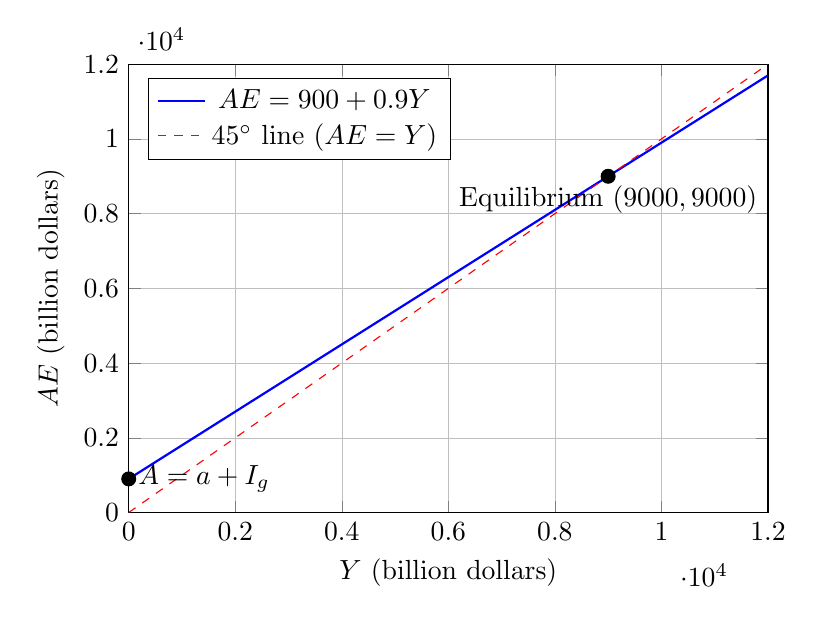
\begin{tikzpicture}
    \begin{axis}[
        width=0.8\textwidth,
        height=0.6\textwidth,
        xlabel={$Y$ (billion dollars)},
        ylabel={$AE$ (billion dollars)},
        xmin=0, xmax=12000,
        ymin=0, ymax=12000,
        xtick={0,2000,4000,6000,8000,10000,12000},
        ytick={0,2000,4000,6000,8000,10000,12000},
        legend pos=north west,
        grid=both,
        grid style={line width=.1pt, draw=gray!30},
        major grid style={line width=.2pt,draw=gray!50},
      ]
      % Plot the AE function: AE = 900 + 0.9Y
      \addplot[
        domain=0:12000,
        samples=100,
        blue,
        thick
      ] {900 + 0.9*x};
      \addlegendentry{$AE = 900 + 0.9Y$}

      % Plot the 45-degree line: AE = Y
      \addplot[
        domain=0:12000,
        samples=100,
        red,
        dashed
      ] {x};
      \addlegendentry{$45 \degree \text{ line } (AE = Y)$}

      % Mark the equilibrium point (9000,9000)
      \addplot[
        only marks,
        mark=*,
        mark size=2.5,
        black
      ] coordinates {(9000,9000)};
      \node[below] at (axis cs:9000,9000) {Equilibrium $(9000,9000)$};

      % Mark y-intercept
      \addplot[
        only marks,
        mark=*,
        mark size=2.5,
        black
      ] coordinates {(0,900)};
      \node[right] at (axis cs:0,900) {$A=a+I_g$};
    \end{axis}
  \end{tikzpicture}
\end{center}

\end{document}
